\chapter{Design}

Once the requirements have been decided, is time to make the design of the system
that will do all needed to cover them. First, we are going to take a look over
the general architecture, the distribution of the domain of the services and
how to delimit their behavior and communications with each other, by after,
take a look to each one to know how to work in each domain and how have been solved all problems
that this design present.

\section{Responsabilites distribution}

At the moment that we decided split the functionality of the system between
services we found the problem that how to decide which is the domain
\intro
At the moment that we decided split the functionality of the system between
services, we found the problem that how to choose which is the domain of each one.
In the majority of the cases, we are beginning from a monolithic system that we
want split, in this instance, is some like this but at first, it was thought to be splited.
\intro
In a common app (whatever kind of it) we have three well-defined layers, user
interface, logic and storage, something as common MVC\footnote{Model–view–controller
(MVC) is a software architectural pattern for implementing user interfaces on
computers. It divides a given application into three interconnected parts in
order to separate internal representations of information from the ways that
information is presented to and accepted from the user, user interfaces pattern,
introduced by Trygve Reenskaug into Smalltalk-76 at Palo Alto Research Center in the 1970s}
A part of user interface make the necessary to present the info and offer the
way to interact with this to the user while the logic layer do this possible
doing the logic steps to work with data structures saved in some kind of storage.
\intro
There are some frameworks as Django wherein all this layer can be developed
together, is not strange their popularity, but if we use other as AngularJS
this only help us in the user interface layer, not in the rest, but for other
hands have another advantage.
\intro
So, that as it may, this would be the more simple schema to start to work in
our domain, with the difference that we work with service instead of layers in a
single program, but essentially, the concept is the same.
\intro
As we can see in the next picture, we will have a user interface, when  will
built all views and controllers that work with this to build a complete user
interface, a logic section layer, here labeled as APIGmService (as a first
approach) that will do the logic of the system, transform the data,
restructuring and offering the interaction form UI to database.
And at end, the database system, mainly an engine of the database and the drivers
necessary to work with them.

\begin{figure}[H]
  \includegraphics[scale=0.25]{img/graphics/initial_microservices_distribution.png}
  \centering
  \caption{Basic layers in common app.}
\end{figure}

\noindent As we can imagine this work fine, is compact and stable when we are talking about
the same code on the same machine but now we are going to split that in
different services, maybe running at different places and maybe in different
languages, so when we talk about divide the domain is about split the logic with
the database access layer.
\intro
Next picture shows us perfectly what are talking about. This is an example
of migration from monolithic to microservices from Nginx resources.

\begin{figure}[H]
  \includegraphics[scale=0.35]{img/graphics/refactoring.png}
  \centering
  \caption{Monolithic to microservices, from nginx resources. }
\end{figure}

\noindent So, for us, each service will always be mainly the same components,
communication protocol and logic layer while database layer will always be optional,
a service can do some logic without need a database, imagine a simple service
to do several calculations or consume the data from another service or act as
third party services gateway, a social network, a payment service, whatever.
\intro
Coming back again to our problem we have decided to split all the back end in
four services that will cover the domain of the problem, following a Domain
Driven Development principles. Each one will be described with details after,
for now, only some reasons that why is so. We need a logic part that controls
any system call, some as the gateway that acts as a dispatcher of requests, that
call to the service (maybe not only one) that can help it to resolve the requests
and give back the info.
\intro
For another and, we need cover all requirements specified,
and to achieve this we are going to design three services that split all logic
issues, it will be \textbf{Teaching Database microService}, \textbf{Students Control}
and \textbf{Analysis microService}. All toguether compose the backend of the app,
toguether with other service that will enlarge the functionality of our project
in the future.
\intro
So, as a big picture, the backend of our service would look like this, some
services with approximately the same form (in the pictur only three, is the same).

\begin{figure}[H]
  \includegraphics[scale=0.25]{img/graphics/backend.png}
  \centering
  \caption{Some as the first approach of the system.}
\end{figure}

\noindent Once that the architecture is clear and the services are well defined
(not their behavior, only their domain) we must have clear how this services will
be deployed in the platform or infrastructure chosen because the selection can
modify the way to design the services.
\intro
So in our case, of all possibilities that we have already discussed before we
only consider two as acceptable, Google and Amazon infrastructure, so as you
know already, Google was the selected, so we need design our services to run
inside of it and this mean that we need how configure our services.
\intro
As we always evaluate some options, we have done a simple design to see what
will be the infrastructure and design required, first in Amazon Web Services.
\intro
In this case, as the code must run into the container we would need configure
all our services as Docker Containers and to use the service Amazon EC2 Container
Service to deploy them. And our gateway service could be deployed in another
container or could be used a specific service called API Gateway Service with
Lambda Service, both services was launched by Amazon when they saw that this
pattern was really common in all projects, and they design this service to save
efforts to developers (even though it have some drawbacks as for example that you
do not try it in local, at least for now but is sure that will be solved).

\begin{figure}[H]
  \includegraphics[scale=0.35]{img/graphics/aws_approach.jpg}
  \centering
  \caption{Approach in Amazon Web Service infrastructure.}
\end{figure}

\noindent The goal of this study was compare the facilities or drawbacks of each platform
(doing a little bit deep study that only to take a look over the solutions each
one offered), and the drawbacks of AWS for this kind of "amateur" project was too.
\intro
Come back to GAE, the deploy must be different because there are not docker
container, we only have speciall sandbox to run our code with some special
characteristics (as wee commented before). But, the architecture does not vary
significantly between both architectures, as could not have been otherwise.
If this not so, microservices and their platform independence would not have sense.
\intro
So, focused on GAE, the services must be deployed and developed (nothing else of
some changes in the code) as modules (now called services by GAE) and this can
(and must) put joined in GAE applications. So, as the platform are thought and
to adjust this to our requirements we are going to launch two apps, one only with
the user web interface service (front end) and another with the group of services
that compound the backend, (here GAE app 2).
You can see the distribution in the next picture.

\begin{figure}[H]
  \includegraphics[scale=0.35]{img/graphics/gae_approach.jpg}
  \centering
  \caption{The same approach in Google App Engine infrastructure.}
\end{figure}


\subsection{Be more realistic}

As is esay to imagine, is needed a lot of services to complete all requirements
of the project, and presented here is only the most important because define the
core of app and their structure but of course are necessary a lot more.
Only thinking about security and authentication is easy to see that is necessary
other services to check this, but as is a standard service (not taking part in
the design of the app) not will be developed now and neither explained here.
Their goals are to ensure the authentication of the user and provide the user
authorization of different parts of the app. So, this will be Authorization \&
Authentication microService.
\intro
On another hand, there are two more functionalities must be developed as soon as
possible in the next iterations, a files storage, and a messaging service.
Both are necessary for a more advanced stage of the deploy, not now, but essential
in the final product. The next picture shows you all services, developed in this
phase and the planned.

\begin{figure}[H]
  \includegraphics[scale=0.22]{img/graphics/final_microservices_distribution.png}
  \centering
  \caption{Group of microservices of SMS launched and planned.}
\end{figure}

\noindent Next picture shows us a more realistic snap of the deployment, with
the services, technologies, tools and third party services consumed.
We can see how SCmS need G Cloud Datastore, TDBmS Cloud SQL (for example) and
all technologies related.

\begin{figure}[H]
  \includegraphics[scale=0.15]{img/graphics/GAE_final_architecture.png}
  \centering
  \caption{Final snap of the distribution of the services with their technologies.}
\end{figure}

\noindent And will be our roadmap to follow, without any service needed to obtain a pre-alfa
product version that satisfy minimum requirements at this point.


\section{API standar status codes}

When we design an API over HTTP we are assuming that we are going to use standard
status code of this protocol (HTTP/1.1 in particular) and is useful that from beginning
all team knows what code will be used and the meaning. The next table shows us which is these,
obviously, there are a lot of more, but this is most important for us.

\begin{table}[H]
\centering

\begin{tabular}{@{}lllllll@{}}

Status Code & Meaning & Use/Behavior\\
\midrule

200 & Ok & Any request that returned content.\\
201 & Created. & Not return content and the item has been saved.\\
204 & Ok without body. & Call with success without content. \\
404 & Not found. & Element not founded.\\
422 & Unprocesable entity. & Bad body at request.\\
500 & Server error. & Any unknown kind of server error.\\

\end{tabular}
\caption{HTTP1.1 Status Code common used}
\label{my-label}
\end{table}

\noindent And as is known, the numbers have a specific meaning and it will
be useful to know just in case another will appear.

\begin{table}[H]
\centering

\begin{tabular}{@{}lllllll@{}}

Class & Meaning\\
\midrule

2xx & Successful\\
3xx & Redirection\\
4xx & Client Error\\
5xx & Server Error\\

\end{tabular}
\caption{HTTP1.1 Status Code first digit meaning}
\label{my-label}
\end{table}


\section{Pesistence Strategy}

When we are talking aobut persitency that meaning how the data that change
their state in the database is manage. Obviously we are talking of the changes
between created, deleted and the between states.
\intro
Is been identified three ways to do this:

\begin{itemize}
  \setlength{\itemsep}{0pt}
\item \textbf{Non persistence}
      \intro
      When a item is updated or deleted any information of the last state remain.
      \intro
\item \textbf{Half persistence}
      \intro
      When a data is logically erased, the data remain in the database but will never
      accesible by the user. In this case is isseful if we want develop some mechanism
      to redo acctions, in this case only deletion actions.
      \intro
\item \textbf{Complete persistence}
      \intro
      When not only the elements erased can be restored, all items can be restored in
      any point of the hisory of the system. This is the more complex mechanism to persistence
      but also the most powerfull and usseful for the users, because as in a simple
      text editor allow do an infinite redo over acctions realized.

\end{itemize}

\noindent Afte study all options have been decided use the second approach, and to achieve
this is necessary get some kind of metadata pluged to our objects stored in databases
to control their state in all moment.
To do this has been designed this metadada pattern for all objects saved in any
service or database:

\begin{lstlisting}[language=python,frame=none]
  Metadata parameters
  createdBy       INT,
  createdAt       DATETIME,
  modifiedBy      INT,
  modifiedAt      DATETIME,
  deletedBy       INT,
  deletedAt       DATETIME,
  deleted         BOOL,

\end{lstlisting}

With it we get a simple way to save logically deleted items, that allow us
develop a simple way to recovery this if user want, and not only this, also
a system to know who do the actions, who save, delete or update an item and
also when, a lot of data very usefull in many ways.


\section{API Gateway microService}

This service has not owned API definition because at this point of development
only takes the role of dispatcher (with a bit logic in some parts, but minimal)
and their only goal is to copy the services API and clone it. Despite this, their
task is very important in the system, talk with clients and with services and thanks
to this nothing of them need to know about another.

\begin{figure}[H]
  \includegraphics[scale=0.35]{img/graphics/apigateway.png}
  \centering
  \caption{Api Gateway service concept.}
\end{figure}

\noindent As it can be seen in the figure above, at first it was designed with Google Cloud
Endpoints technology, using Python and gRPC but, as we will explain in the next
chapter, was not the best way (at least with the system that we can build) and
finally was decided to build as the rest of them, using Flak and building a
simple and well know API Rest.


\section{Teaching Data Base microService}

\subsection{Domain and design}

This mService offers the managment of the teaching of the center.
This means that persist in a relational database all relations between
teachers, students, subjects, etc, and all resource availables to
make this posible throuhg an api.
\intro
This like the rest offers his resource throuhg an api writed in Flask
(follow the same architecture that all).
\intro
The engine to save all these relations is MySQL, for many reasons,
mainly because is the best known engine and in which it has some experience
and also because GCP offers as a cloud product Google Cloud SQL Databases.
Until recently only offerts MySQL but now (since March of 2017) they
offer also PostgreSQL.
\intro
In the old version it was a little ORM that offers simple methods
to access data transform this in SQL raw sencentes. Now this library
is only a wraper of the SQLAlchemy to keep apart the apirest of the
service to the database access layer.

\begin{figure}[H]
  \includegraphics[scale=0.35]{img/graphics/tdbms.png}
  \centering
  \caption{Teaching Data Base service parts.}
\end{figure}


\subsection{Api definition}

To get API definitions will be used  RAML\footnote{ RESTful API Modeling Language
(RAML) was launched at 2013 and is YAML based language for describing RESTful APIs }.
In spite of to be more powerful, it only will be used to do a good definition of the
APIs independently of the technology with after it will be developed, understandable
for any developer.
\intro
In this case, the API definition of this service is like this, and as we can see,
is very easy to understand, and we only are going to use the most simple
version of this definition standard, there a lot of other things that we can
express, but is not necesary as first approach.





\subsection{Database logical design}

Based on user histories and the domain of the problem the designe
done based of this entity relation diagram:
\intro
The design follow some details that the domain presents, that is related
(at least the more significantly) below:

\begin{figure}[H]
  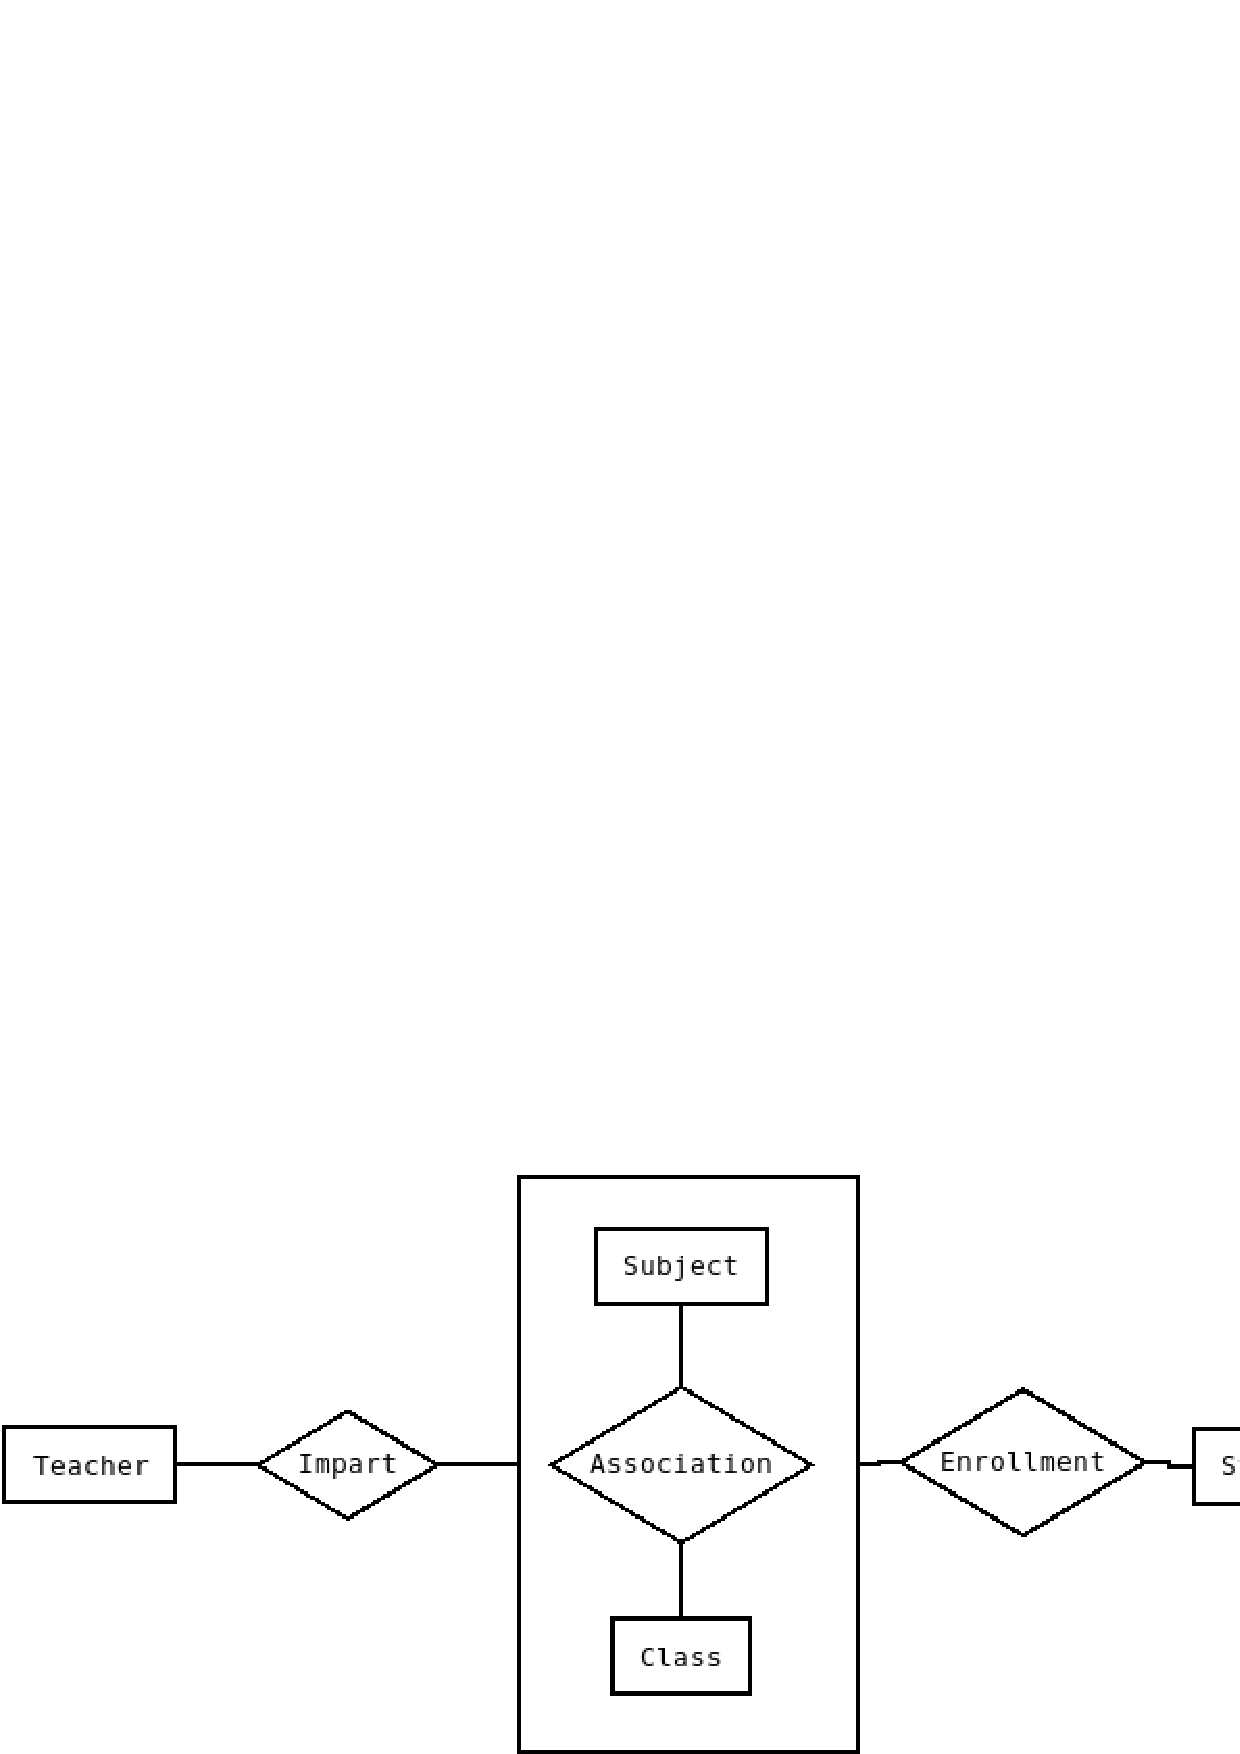
\includegraphics[scale=0.4]{img/diagrams/dbms-ER.png}
  \centering
  \caption{Entity-Relationship Diagram.}
\end{figure}


\subsubsection{Data model}
\begin{lstlisting}[language=python,frame=none]
  CREATE TABLE student (
    studentId       INT NOT NULL AUTO_INCREMENT,
    name            CHAR(100) NOT NULL,
    surname         CHAR(100) NOT NULL,
    dni             INT,
    email           CHAR(120),
    address         CHAR(100),
    locality        CHAR(50),
    province        CHAR(50),
    birthdate       DATE,
    phone           CHAR(50),
    profileImageUrl CHAR(200),
    gender          CHAR(1),

    #Metadata parameters
    createdBy       INT,
    createdAt       DATETIME,
    modifiedBy      INT,
    modifiedAt      DATETIME,
    deletedBy       INT,
    deletedAt       DATETIME,
    deleted         BOOL,

    PRIMARY KEY (studentId),
    UNIQUE (dni, deleted)
  );
\end{lstlisting}

\begin{lstlisting}[language=python,frame=none]
  CREATE TABLE teacher (
    teacherId       INT NOT NULL AUTO_INCREMENT,
    name            CHAR(100) NOT NULL,
    surname         CHAR(100) NOT NULL,
    dni             INT,
    email           CHAR(120),
    address         CHAR(100),
    locality        CHAR(50),
    province        CHAR(50),
    birthdate       DATE,
    phone           CHAR(50),
    profileImageUrl CHAR(200),
    gender          CHAR(1)

    #Metadata parameters
    createdBy       INT,
    createdAt       DATETIME,
    modifiedBy      INT,
    modifiedAt      DATETIME,
    deletedBy       INT,
    deletedAt       DATETIME,
    deleted         BOOL,

    PRIMARY KEY (teacherId),
    UNIQUE (dni, deleted)
  );
\end{lstlisting}


\begin{lstlisting}[language=python,frame=none]
  CREATE TABLE subject (
    subjectId   INT NOT NULL AUTO_INCREMENT,
    name        CHAR(100) NOT NULL,
    description CHAR(255),

    #Metadata parameters
    createdBy   INT,
    createdAt   DATETIME,
    modifiedBy  INT,
    modifiedAt  DATETIME,
    deletedBy   INT,
    deletedAt   DATETIME,
    deleted     BOOL,

    PRIMARY KEY (subjectId),
    UNIQUE (name, deleted)
  );
\end{lstlisting}

\begin{lstlisting}[language=python,frame=none]
  CREATE TABLE class (
    classId    INT NOT NULL AUTO_INCREMENT,
    course     INT(1) NOT NULL,
    word       CHAR(10) NOT NULL,
    level      CHAR(20) NOT NULL,
    description CHAR(255),

    #Metadata attributes
    createdBy  INT,
    createdAt  DATETIME,
    modifiedBy INT,
    modifiedAt DATETIME,
    deletedBy  INT,
    deletedAt  DATETIME,
    deleted    BOOL,

    PRIMARY KEY (classId),
    UNIQUE (course, word, level, deleted)
  );
\end{lstlisting}

\begin{lstlisting}[language=python,frame=none]
  CREATE TABLE association (
    associationId INT NOT NULL AUTO_INCREMENT,
    classId       INT,
    subjectId     INT,

    #Metadata parameters
    createdBy     INT,
    createdAt     DATETIME,
    modifiedBy    INT,
    modifiedAt    DATETIME,
    deletedBy     INT,
    deletedAt     DATETIME,
    deleted       BOOL,

    FOREIGN KEY (subjectId) REFERENCES subject (subjectId),
    FOREIGN KEY (classId) REFERENCES class (classId),
    PRIMARY KEY (associationId),
    UNIQUE (subjectId, classId, deleted)
  );
\end{lstlisting}

\begin{lstlisting}[language=python,frame=none]
CREATE TABLE impart (
  impartId      INT NOT NULL AUTO_INCREMENT,
  associationId INT,
  teacherId     INT,

  #Metadata parameters
  createdBy     INT,
  createdAt     DATETIME,
  modifiedBy    INT,
  modifiedAt    DATETIME,
  deletedBy     INT,
  deletedAt     DATETIME,
  deleted       BOOL,

  FOREIGN KEY (associationId) REFERENCES association (associationId),
  FOREIGN KEY (teacherId) REFERENCES teacher (teacherId),
  PRIMARY KEY (impartId),
  UNIQUE (associationId, teacherId, deleted)
);
\end{lstlisting}

\begin{lstlisting}[language=python,frame=none]
CREATE TABLE enrollment (
  enrollmentId  INT NOT NULL AUTO_INCREMENT,
  studentId     INT,
  associationId INT,

  #Metadata parameters
  createdBy     INT,
  createdAt     DATETIME,
  modifiedBy    INT,
  modifiedAt    DATETIME,
  deletedBy     INT,
  deletedAt     DATETIME,
  deleted       BOOL,

  FOREIGN KEY (associationId) REFERENCES association (associationId),
  FOREIGN KEY (studentId) REFERENCES student (studentId),
  PRIMARY KEY (enrollmentId),
  UNIQUE (studentId, associationId, deleted)
);
\end{lstlisting}





\subsection{Way to access to raw data}

While at firs of develop the mainly strategie to follow was write
all by cero, finally the point of view has been changed to follow
the use of standard tools and avoid reinvent the wheel.
\intro
So, if in the first stages of the project the acces to raw data through
the engine was hand made, using an own simple library that worked
like as a simple ORM\footnote{Object-relational mapping or \textbf{ORM} is a
technique for converting data between incompatible
type systems using oriented objects pogramation to do this, as for example access
to database systems}, the evolution of it and especially the problems
found and the unmaintainability of code have made that now the approach
turned to use a good tool as ORM like SQLAlchemy\footnote{}.
\intro
The changes in the specifications of the api while the develop and
the maintaince of the performance of the queries when is writed hand
made in raw SQL isn't a good idea. Before the develop of this mService
it easy to understand that only in few projects is justified the use
of raw sql sencences and drivers whiout ORM (by easy that it was).


\section{Students Control microService}

\subsection{Domain and design}

\begin{figure}[H]
  \includegraphics[scale=0.4]{img/graphics/scms.png}
  \centering
  \caption{Students Control service parts.}
\end{figure}

\subsection{Api definition}

How was commented before, the design of the resources is based on getting an user
interface with minimal requirements. So, there are a lot of ways to get a collection
of data to present it on the interface, and we must decide who do the more complex
part of this compose, and obviously, we want to save time to the user device.
To better understand it, is best an example. If we want to get a list of attendance
controls that have been done and if we only request the raw list we only will
obtain a list with all data but without any reference to the data of teacher of
data of the subject.
\intro
So, to can offer by the user interface all data that it need,   is necessary to
develop the fill of this data before to send. And all this complexity must be a
backend issue, indecently of the request or the mechanism that this use.
We can see an example of this in \textit{ac resource} when is called with
\textit{GET} method.


\subsubsection{Attendance Controls API Subsection}
The sub API which we can manage all related with attendance controls, that are
records about the attendance of the students to class and something as if the
students attends with delay, if this is justified, if gone with or without
the uniform, etc. As with the previous, this is the behavior designed RAML based.


\subsubsection{Disciplinary Notes API Subsection}

With this API section, we can manage all related with disciplinary notes, that
are records about the student's behavior in class. With this we can to register
negative acts of the students to prevent big problems and to correct this as soon
as possible. And this is the behavior designed RAML based.


\subsubsection{Maks API Subsection}

As the final part of the simple student control that we do we still have the marks
section.  With this we would record all exams marks that students achieve, that
is another big part that was required. As with the previous, this is the
behavior designed RAML based.


\section{User Interface microService}

\subsection{Domain and design}

As has been mentioned, we are going to use AngularJS to build the user interface.
This means that the files of the app would be load from a service to user devices
and from there it will make all requests to the server, so the single purpose of
the service is to serve all app files.
The design follows bellow schema.

\begin{figure}[H]
  \includegraphics[scale=0.4]{img/graphics/ui.png}
  \centering
  \caption{User interface service logic.}
\end{figure}


\subsubsection{About design}

All the designe of the app is based of Java Script files. And the structure will
be this,  a section o Students Control where will placed all sections related,
as Attendance Controls, Discipline, and Marks section and another section, the
biggest, with all related with the teaching as can be all sections that the domain
has, teachers, students, subjects, classes, and the rest of items related.
\intro
The most of the parts need the same javascript files, controllers to define the
logic and services to interact with the server. Moreover as the idea is work as
each logical part as independly modules they will be built as modules as well.
\intro
This is the wireframes that give an approach of the design that we want for
our interface. There are a lot of parts, sections and detail that will
filled houndred of pages, so this is some examples of the simple a common
parte as work with list, in this case of teachers.

\subsubsection{About distribution}

The design of the components of the interface will follow
Google Material Design Philosofy\footnote{Google announced Material Design on
June, 2014, at Google I/O conference}, it is a design language developed by
Google.

\begin{figure}[H]
  \includegraphics[scale=0.4]{img/graphics/MaterialDesign.png}
  \centering
  \caption{Some typical Material Design UI components.}
\end{figure}

\noindent To objtain this characteristic designe there are a lot of options, but easiest
is to use some CSS Framework existing instead of try to implement our own
css components. There are some options availables, as \textit{Materialize},
\textit{MUI}, \textit{Material UI}, \textit{Polymer} (that is much moret),
we could talk about it hours, and \textit{Angular Material}, that is which
we are selected.
Why? because is not only a css kit, is a group of Angular directives that allow
us to use their css components as directives, some very powerfull and simple,
that increase the speed of develop when their behaviour is well understood.
\intro
Indenpendly of the style guide that we use we need design the interface,
their parts, the position of the elements and how interact this among them and
amoung several screens of our app.
To do this design most common way is use a system of wireframing, that is
as a way to compound user interfaces using very abstract form, puting the
focus in the position and general design instead of the details, colors, or
somethings like this.
There are some tools to do this, all do basically the same, and we
are going to use Pencil (An open-source GUI prototyping tool that's available
for all platforms).
\intro
We would need a dozen of pages to show all sections of app. Bellow it can see
some example of design with two samples of teachers section,
that it will follow in the rest of the design, that possibly will suffer some
change in the way.

\begin{figure}[H]
  \includegraphics[scale=0.2]{img/snaps/teachers_list_wireframe.png}
  \centering
  \caption{Teachers List view wireframed.}
\end{figure}

\begin{figure}[H]
  \includegraphics[scale=0.2]{img/snaps/teacher_profile_wireframe.png}
  \centering
  \caption{Teacher profile view wireframed.}
\end{figure}

\noindent The rest of them have been handmade (on paper) and it was believed unnecessary
to include all digital wireframes here.

\section{Analysis microService}

The goal of this service is easy, we need a centered way to can retrieve reports
of all of our relevant kind of items in the app, as courses, classes, teachers and
mostespecially, of students.
If we think only in simple reports maybe is not necessarily an independent service
that offers that (only this is enough interesting the services to manage the
relations keep their simplicity) but if we think in report that included statistics
and data analysis as regresion, trends and alert detection in students behavior
the scenario changes completely.
\intro
To do this we need to use some specific tools,
libraries, and techniques which have little to do with  the domains of the rest
of services. Moreover of this, to achieve some of the conclusion that this service
will obtain will be necessary cross data between services, so externalize this in
another actor in the system is more reasonable.

\subsection{Domain and design}

Logically, this service follow the same design of the rest. A library that wraps
the complexity of the logic is accessed by a standard API (as the rest as well).
The main difference is that the database used in this case is TinyDB\footnote{More
info about the system here: https://pypi.python.org/pypi/tinydb}, a lightweight
document oriented database, written in pure Python (without external dependencies).
\intro
This was chosen for a simple reason, we need some storage system to save the data
calculated to avoid do them again for each request, and as is a service that not
store a big amount of data is a good option and really easy to implement.
The picture below show the logic of the service.

\begin{figure}[H]
  \includegraphics[scale=0.3]{img/graphics/ams.png}
  \centering
  \caption{Teacher profile view wireframed.}
\end{figure}

\noindent Our goal with this service is can get obtain more complex data that the services
can offer us to can offer to the user interface good data blocks to build powerful
graphics.  As in the domain that we are the students have been evaluated by
competencies in addition to particular subject skills and knowledge the app must
offer some way to can check these competencies at general scope (independently of
the subject) and this kind of information is perfect to use (among others)
\textit{polar charts as these}:

\begin{figure}[H]
  \includegraphics[scale=0.45]{img/graphics/polar.png}
  \centering
  \caption{Subjects and competences polar charts.}
\end{figure}

\noindent In these, we can see as a specific student has their competencies covered and
what it need to improve and the same with the subjects, not only in this course
or semester, also comparing with previous of futures using simple regression
equations. We can imagine the power of this kind of shots of data by the educators
of the center, that would require a lot of work if they would do handmade.


\begin{figure}[H]
  \includegraphics[scale=0.47]{img/graphics/evolution.png}
  \centering
  \caption{Subjects and competences polar charts.}
\end{figure}

\noindent Not is the goal review all possibilities of data flow that it can be exploited
with all items and their relations, but the above picture shows another interesting
bunch of data well presented to be analyzed by an educator. As we save all things
that a student do in the center, homework, marks, behavior, delays, etc. We can build
a points system that in a range of 0 to 100, we can measure the efficiency of the
student per week. That means that if a student does all their homework, all their
exams well, without any delay, etc. It will be 100 points in this week and the
opposite if it does not do anything.
\intro
It is mighty because in a look we can know how the student is, how is their
evolution and the best interesting (using simple regression) which is their trend,
to be able to make decisions proactively, not when will be too late, improving
drastically the way to understand the student tracking systems.
\textbf{And it is only the begin}.

\subsection{API Definition}

In this case, the API is very small (not meaning nothing) because is not few
relations between items inside, we only need a way to request reports to the
system, nothing else.



\section{Auxiliar tools}

\subsection{Provisioner}
A provisioner is simply a tool used to provide a system to insert test data, to
avoid to do this hand-made, in our services.

\begin{center}
\includegraphics[scale=0.4]{img/graphics/provisioner.png}
\end{center}

\noindent Normally this work without knowledge
of the internal parts of the backend, only working with their API gateway (or
API if we want only fill the database of service), understanding it as a black box.
this is only an approach, we can design our provisioner to fill data directly
in the databases, which will require established a connection with them without
the interaction of the services or their connection libraries. This is faster but
on some occasions, we do not want to do this, because another of their goal is to
check at the same time the correctly of all parts of APIs involved in the data insertion.
\intro
So, the execution this kind of program required that the system has fully launched.
This will be the most used tool when we want to try some feature that required a
lot of data in the system.
\intro
How does it work? Easy, only need simple parameters as entry and based on some rules it will do all
calls to the API gateway to insert all data required, besides to save all operations
in a register or log file because is necessary to check this in a debug operation.

\subsection{Data base helpers and testing tools}

To all those repetitive tasks as clean the database, create it, populate or
something like this, reinstall the engine or purge of the system we will need
some scripts to help us and will be necessary develop this.
\intro
About the testing tools, side server will be enough with the normal testing using
pytests (we could talk a lot of it) and over user interface, we would be using
Selenium\footnote{Know more at: http://www.seleniumhq.org/},
in words of their creators, textit{it is for automating web applications for
testing purposes but is certainly not limited to just that}.
\intro
Thinking of this pair of details, we would have covered all design decision taken,
ready to start do develop, crossing the fingers to get all in time.
